\documentclass{standalone}
\usepackage{tikz}
\usetikzlibrary{patterns, positioning}


\begin{document}
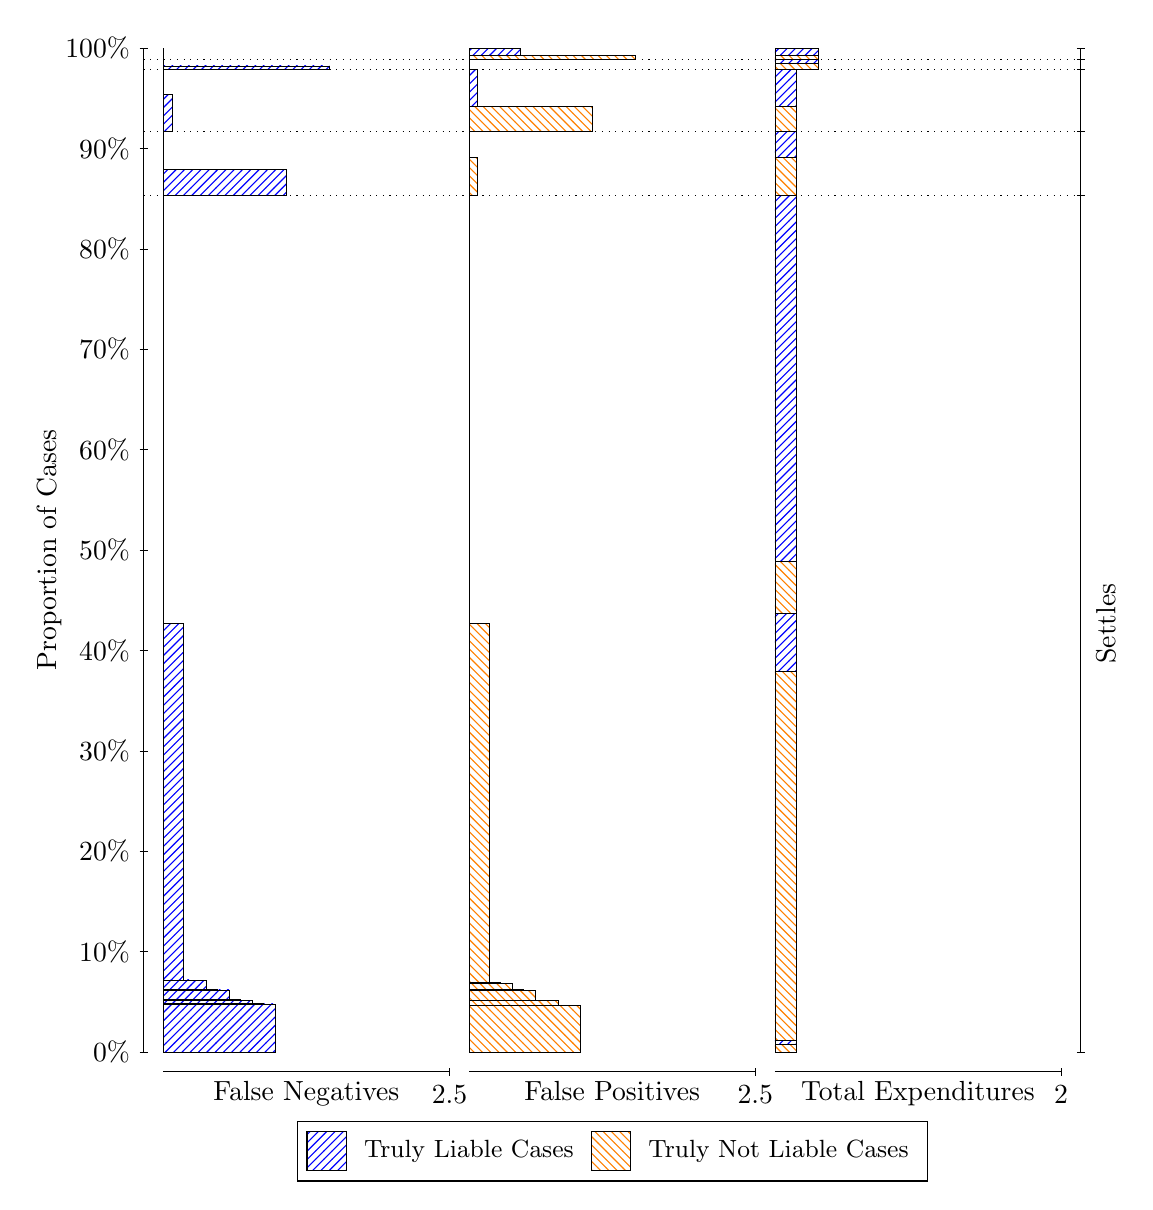
\begin{tikzpicture}
\draw[black, very thin] (1.5,1.75) -- (1.5,14.5);
\node[rotate=90, text=black, anchor=center] at (0.3, 8.125) {Proportion of Cases};
\draw[black, very thin] (1.45,1.75) -- (1.55,1.75);
\node[text=black, anchor=east] at (1.45, 1.75) {0\%};
\draw[black, very thin] (1.45,3.025) -- (1.55,3.025);
\node[text=black, anchor=east] at (1.45, 3.025) {10\%};
\draw[black, very thin] (1.45,4.3) -- (1.55,4.3);
\node[text=black, anchor=east] at (1.45, 4.3) {20\%};
\draw[black, very thin] (1.45,5.575) -- (1.55,5.575);
\node[text=black, anchor=east] at (1.45, 5.575) {30\%};
\draw[black, very thin] (1.45,6.85) -- (1.55,6.85);
\node[text=black, anchor=east] at (1.45, 6.85) {40\%};
\draw[black, very thin] (1.45,8.125) -- (1.55,8.125);
\node[text=black, anchor=east] at (1.45, 8.125) {50\%};
\draw[black, very thin] (1.45,9.4) -- (1.55,9.4);
\node[text=black, anchor=east] at (1.45, 9.4) {60\%};
\draw[black, very thin] (1.45,10.675) -- (1.55,10.675);
\node[text=black, anchor=east] at (1.45, 10.675) {70\%};
\draw[black, very thin] (1.45,11.95) -- (1.55,11.95);
\node[text=black, anchor=east] at (1.45, 11.95) {80\%};
\draw[black, very thin] (1.45,13.225) -- (1.55,13.225);
\node[text=black, anchor=east] at (1.45, 13.225) {90\%};
\draw[black, very thin] (1.45,14.5) -- (1.55,14.5);
\node[text=black, anchor=east] at (1.45, 14.5) {100\%};

\draw[black, very thin] (13.4,1.75) -- (13.4,14.5);
\draw[black, very thin] (13.35,1.75) -- (13.45,1.75);
\node[anchor=west] at (13.35, 1.75) {};
\draw[black, very thin] (13.35,12.632) -- (13.45,12.632);
\node[anchor=west] at (13.35, 12.632) {};
\draw[black, very thin] (13.35,13.439) -- (13.45,13.439);
\node[anchor=west] at (13.35, 13.439) {};
\draw[black, very thin] (13.35,14.224) -- (13.45,14.224);
\node[anchor=west] at (13.35, 14.224) {};
\draw[black, very thin] (13.35,14.359) -- (13.45,14.359);
\node[anchor=west] at (13.35, 14.359) {};
\draw[black, very thin] (13.35,14.5) -- (13.45,14.5);
\node[anchor=west] at (13.35, 14.5) {};

\draw[black, very thin, pattern color=blue, pattern=north east lines] (1.75,1.75) rectangle (3.167,2.3613);
\draw[black, very thin, pattern color=blue, pattern=north east lines] (1.75,2.3613) rectangle (3.0217,2.3651);
\draw[black, very thin, pattern color=blue, pattern=north east lines] (1.75,2.3651) rectangle (2.8763,2.4067);
\draw[black, very thin, pattern color=blue, pattern=north east lines] (1.75,2.4067) rectangle (2.731,2.4134);
\draw[black, very thin, pattern color=blue, pattern=north east lines] (1.75,2.4134) rectangle (2.5857,2.5378);
\draw[black, very thin, pattern color=blue, pattern=north east lines] (1.75,2.5378) rectangle (2.4403,2.5477);
\draw[black, very thin, pattern color=blue, pattern=north east lines] (1.75,2.5477) rectangle (2.295,2.6576);
\draw[black, very thin, pattern color=blue, pattern=north east lines] (1.75,2.6576) rectangle (2.1497,2.6669);
\draw[black, very thin, pattern color=blue, pattern=north east lines] (1.75,2.6669) rectangle (2.0043,7.1903);
\draw[black, very thin, pattern color=orange, pattern=north west lines] (1.75,7.1903) rectangle (1.75,12.632);
\draw[black, very thin, pattern color=blue, pattern=north east lines] (1.75,12.632) rectangle (3.3123,12.957);
\draw[black, very thin, pattern color=orange, pattern=north west lines] (1.75,12.957) rectangle (1.75,13.439);
\draw[black, very thin, pattern color=blue, pattern=north east lines] (1.75,13.439) rectangle (1.859,13.908);
\draw[black, very thin, pattern color=orange, pattern=north west lines] (1.75,13.908) rectangle (1.75,14.224);
\draw[black, very thin, pattern color=blue, pattern=north east lines] (1.75,14.224) rectangle (3.8573,14.273);
\draw[black, very thin, pattern color=orange, pattern=north west lines] (1.75,14.273) rectangle (1.75,14.359);
\draw[black, very thin, pattern color=orange, pattern=north west lines] (1.75,14.359) rectangle (1.75,14.409);
\draw[black, very thin, pattern color=blue, pattern=north east lines] (1.75,14.409) rectangle (1.75,14.5);
\draw[black, very thin, pattern color=orange, pattern=north west lines] (5.6333,1.75) rectangle (7.0503,2.341);
\draw[black, very thin, pattern color=orange, pattern=north west lines] (5.6333,2.341) rectangle (6.905,2.3458);
\draw[black, very thin, pattern color=orange, pattern=north west lines] (5.6333,2.3458) rectangle (6.7597,2.4027);
\draw[black, very thin, pattern color=orange, pattern=north west lines] (5.6333,2.4027) rectangle (6.6143,2.4093);
\draw[black, very thin, pattern color=orange, pattern=north west lines] (5.6333,2.4093) rectangle (6.469,2.5323);
\draw[black, very thin, pattern color=orange, pattern=north west lines] (5.6333,2.5323) rectangle (6.3237,2.5339);
\draw[black, very thin, pattern color=orange, pattern=north west lines] (5.6333,2.5339) rectangle (6.3237,2.5437);
\draw[black, very thin, pattern color=orange, pattern=north west lines] (5.6333,2.5437) rectangle (6.1783,2.6234);
\draw[black, very thin, pattern color=orange, pattern=north west lines] (5.6333,2.6234) rectangle (6.033,2.6308);
\draw[black, very thin, pattern color=orange, pattern=north west lines] (5.6333,2.6308) rectangle (5.8877,7.1916);
\draw[black, very thin, pattern color=blue, pattern=north east lines] (5.6333,7.1916) rectangle (5.6333,12.632);
\draw[black, very thin, pattern color=orange, pattern=north west lines] (5.6333,12.632) rectangle (5.7423,13.114);
\draw[black, very thin, pattern color=blue, pattern=north east lines] (5.6333,13.114) rectangle (5.6333,13.439);
\draw[black, very thin, pattern color=orange, pattern=north west lines] (5.6333,13.439) rectangle (7.1957,13.754);
\draw[black, very thin, pattern color=blue, pattern=north east lines] (5.6333,13.754) rectangle (5.7423,14.224);
\draw[black, very thin, pattern color=orange, pattern=north west lines] (5.6333,14.224) rectangle (5.6333,14.309);
\draw[black, very thin, pattern color=blue, pattern=north east lines] (5.6333,14.309) rectangle (5.6333,14.359);
\draw[black, very thin, pattern color=orange, pattern=north west lines] (5.6333,14.359) rectangle (7.7407,14.409);
\draw[black, very thin, pattern color=blue, pattern=north east lines] (5.6333,14.409) rectangle (6.2873,14.5);
\draw[black, very thin, pattern color=orange, pattern=north west lines] (9.5167,1.75) rectangle (9.7892,1.8484);
\draw[black, very thin, pattern color=blue, pattern=north east lines] (9.5167,1.8484) rectangle (9.7892,1.9005);
\draw[black, very thin, pattern color=orange, pattern=north west lines] (9.5167,1.9005) rectangle (9.7892,6.5844);
\draw[black, very thin, pattern color=blue, pattern=north east lines] (9.5167,6.5844) rectangle (9.7892,7.3201);
\draw[black, very thin, pattern color=orange, pattern=north west lines] (9.5167,7.3201) rectangle (9.7892,7.9794);
\draw[black, very thin, pattern color=blue, pattern=north east lines] (9.5167,7.9794) rectangle (9.7892,12.632);
\draw[black, very thin, pattern color=orange, pattern=north west lines] (9.5167,12.632) rectangle (9.7892,13.114);
\draw[black, very thin, pattern color=blue, pattern=north east lines] (9.5167,13.114) rectangle (9.7892,13.439);
\draw[black, very thin, pattern color=orange, pattern=north west lines] (9.5167,13.439) rectangle (9.7892,13.754);
\draw[black, very thin, pattern color=blue, pattern=north east lines] (9.5167,13.754) rectangle (9.7892,14.224);
\draw[black, very thin, pattern color=orange, pattern=north west lines] (9.5167,14.224) rectangle (10.062,14.309);
\draw[black, very thin, pattern color=blue, pattern=north east lines] (9.5167,14.309) rectangle (10.062,14.359);
\draw[black, very thin, pattern color=orange, pattern=north west lines] (9.5167,14.359) rectangle (10.062,14.409);
\draw[black, very thin, pattern color=blue, pattern=north east lines] (9.5167,14.409) rectangle (10.062,14.5);
\draw[black, dotted] (1.5,12.632) -- (13.4,12.632);
\draw[black, dotted] (1.5,13.439) -- (13.4,13.439);
\draw[black, dotted] (1.5,14.224) -- (13.4,14.224);
\draw[black, dotted] (1.5,14.359) -- (13.4,14.359);
\draw[black, very thin] (1.75,1.5) -- (5.3833,1.5);
\node[text=black, anchor=north] at (3.5667, 1.5) {False Negatives};
\draw[black, very thin] (5.3833,1.45) -- (5.3833,1.55);
\node[text=black, anchor=north] at (5.3833, 1.45) {2.5};

\draw[black, very thin] (5.6333,1.5) -- (9.2667,1.5);
\node[text=black, anchor=north] at (7.45, 1.5) {False Positives};
\draw[black, very thin] (9.2667,1.45) -- (9.2667,1.55);
\node[text=black, anchor=north] at (9.2667, 1.45) {2.5};

\draw[black, very thin] (9.5167,1.5) -- (13.15,1.5);
\node[text=black, anchor=north] at (11.333, 1.5) {Total Expenditures};
\draw[black, very thin] (13.15,1.45) -- (13.15,1.55);
\node[text=black, anchor=north] at (13.15, 1.45) {2};

\node[text=black, centered, rotate=90] at (13.72, 7.191) {Settles};





\draw (7.449999999999999,1.5) node[draw=none] (baseCoordinate) {};
\begin{scope}[align=center]
        \matrix[scale=0.5, draw=black, below=0.5cm of baseCoordinate, nodes={draw}, column sep=0.1cm]{
            \node[rectangle, draw, minimum width=0.5cm, minimum height=0.5cm, pattern color=blue, pattern=north east lines] {}; &
            \node[draw=none, font=\small, text=black] (B) {Truly Liable Cases}; &
            \node[rectangle, draw, minimum width=0.5cm, minimum height=0.5cm, pattern color=orange, pattern=north west lines] {}; &
            \node[draw=none, font=\small, text=black] (B) {Truly Not Liable Cases}; \\
            };
\end{scope}

\end{tikzpicture}
\end{document}